% 来源：固定来源 PDF（2004福建文.pdf）第 1 页（印刷页 166）Q10 球面截面示意图
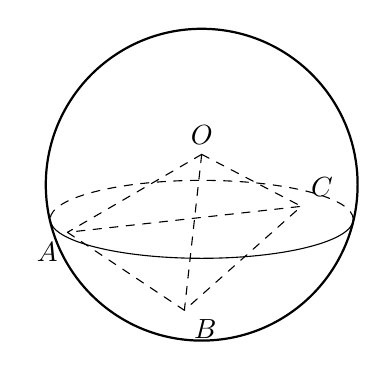
\begin{tikzpicture}[scale=1.1, line cap=round, line join=round]
  % 球体轮廓
  \draw[thick] (0, 0) circle (1.8);

  % 截面圆轮廓（前实后虚）
  \draw[dashed, thin] (1.75, -0.4) arc[start angle=0, end angle=180, x radius=1.75, y radius=0.45];
  \draw[thin] (-1.75, -0.4) arc[start angle=180, end angle=360, x radius=1.75, y radius=0.45];

  % 关键点坐标
  \coordinate (O) at (0, 0.35);
  \coordinate (A) at (-1.55, -0.55);
  \coordinate (B) at (-0.2, -1.45);
  \coordinate (C) at (1.15, -0.25);

  % 三角形 ABC 虚线
  \draw[dashed] (A) -- (B) -- (C) -- cycle;

  % OA, OB, OC 连线虚线
  \draw[dashed] (O) -- (A);
  \draw[dashed] (O) -- (B);
  \draw[dashed] (O) -- (C);

  % 顶点标注
  \node[above] at (O) {$O$};
  \node[below left] at (A) {$A$};
  \node[below right] at (B) {$B$};
  \node[above right] at (C) {$C$};
\end{tikzpicture}
